\documentclass{article}

\usepackage[utf8]{inputenc}
\usepackage{braket}
\usepackage{enumitem}
\usepackage{multirow}
\usepackage{xcolor}
\usepackage[T1]{fontenc}
% \usepackage[french]{babel}
\usepackage{amssymb}
\usepackage{mathtools}
\usepackage{ntheorem}
\usepackage{amsmath}
\usepackage{amssymb}
\usepackage[ a4paper, hmargin={2cm, 2cm}, vmargin={2cm, 2cm}]{geometry}
\usepackage{capt-of}

\usepackage{tikz}
\usetikzlibrary{arrows}
\usetikzlibrary{angles,quotes}

\theoremstyle{plain}
\theorembodyfont{\normalfont}
\theoremseparator{~--}
\newtheorem*{define}{Definition}%[section]
\newtheorem*{ex}{Example}%[section]
\newtheorem*{exe}{Exercise}%[section]
\newtheorem*{obs}{Observation}%[section]
\newtheorem*{remk}{Remark}%[section]
\newtheorem*{nota}{Notation}%[section]
\newtheorem*{fact}{Fact}%[section]
\newtheorem*{claim}{Claim}%[section]
\newtheorem*{supo}{Suppose}%[section]

\newcommand{\norm}[1]{\left\lVert#1\right\rVert}

\usepackage{hyperref}
\hypersetup{
    colorlinks,
    citecolor=black,
    filecolor=black,
    linkcolor=blue,
    urlcolor=blue
}

\title{Lambda Calculus and category theory}
\author{Valeran MAYTIE}
\date{}

\begin{document}
  \maketitle

  \tableofcontents

  \section{Introduction}

  \paragraph{Boole} :
    \begin{itemize}
      \item
        If you consider propositions (no quantifiers) of
        \underline{classical logic} : $A ::= P | A \wedge B | \neg A | A \wedge B |
        \top | \bot $
      \item
        \underline{Ordered} by logical implication $A \leq B \Leftrightarrow A
        \Rightarrow B$, $A$ implies $B$ or $A \vdash B$
    \end{itemize}

    \underline{Observation} $A \wedge B \leq A, A \wedge B \leq B$. moreover if
    $C \leq A$ and $C \leq B$ then $C \leq A \wedge B$ (for all proprieties)

    Which means that $A \wedge B$ define a infimum of $A$ and $B$ (greatest lower
    bound, or \underline{glb})

  \define $A \Rightarrow B = (\neg A) \vee B = \neg (A \wedge \neg B)$.

  \hspace{5mm}

  Observation : \begin{itemize}
    \item $A \wedge (A \Rightarrow B) \leq B$
    \item $A \vee \neg A \leq \text{true}$
    \item $A \wedge \neg A \geq \text{false}$
  \end{itemize}\paragraph{Frege} Ideography (first proof system)

  The idea that a mathematical proof is a mathematical object. In particular
  there may be different proofs of a proposition $A$ formula.


  \begin{center}
  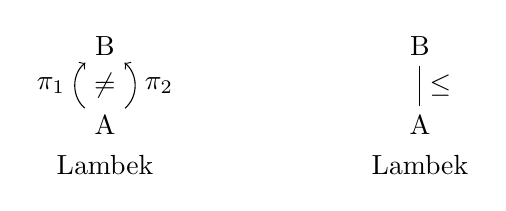
\begin{tikzpicture}
    \node (A) at (-2, 0) {A};
    \node (B) at (-2, 1) {B};
    \node at (-2, 0.5) {$\not =$};

    \draw[->] (A) to [bend right=50] node [right] {$\pi_2$} (B);
    \draw[->] (A) to [bend left=50]  node [left ] {$\pi_1$} (B);

    \node at (-2, -0.5) {Lambek};

    \node (A) at (2, 0) {A};
    \node (B) at (2, 1) {B};

    \draw (A) to node [right] {$\leq$} (B);
    \node at (2, -0.5) {Lambek};

  \end{tikzpicture}
  \end{center}


  Lambek understood connection between:

  \begin{center}
  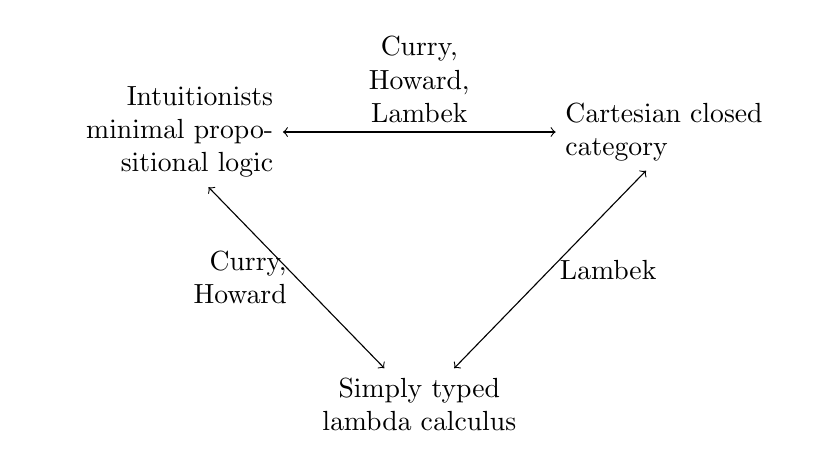
\begin{tikzpicture}
    \node[text width=3cm, anchor=west] (Cat) at (30:2) {Cartesian closed category};
    \node[text width=3cm, align=right, anchor=east] (Log) at (150:2) {Intuitionists minimal propositional logic};
    \node[text width=3cm, align=center, anchor=north] (Lam) at (270:2) {Simply typed lambda calculus};

    \draw [<->] (Cat) edge node[above, text width=2cm, align=center] {Curry, Howard, Lambek} (Log);
    \draw [<->] (Cat) edge node[right] {Lambek} (Lam);
    \draw [<->] (Log) edge node[left, text width=2cm, align=right] {Curry, Howard} (Lam);
  \end{tikzpicture}
  \end{center}

  \define A monoid $(M, \bullet, e)$ is a set $M$ equipped with a binary
  operation $\bullet : M \times M \to M$ with a neutral element $e \in M_e : M^0
  \to M$ satisfying two equations :

  \begin{itemize}
    \item (associativity) $\forall x, y, z \in M, x \bullet (y \bullet z) = (x
      \bullet y) \bullet z$
    \item (neutrality) $\forall x, \in M, x \bullet e = x = e \bullet x$
  \end{itemize}

  \ex $(\mathbb N, +, 0), (\mathbb Z, +, 0), (\mathbb N, \times, 1)$ and any
  group.

  Free monoid on a set (=alphabet) $A$. % todo: phrase qui veut rien dire ici
  $A^*$ contains finite sequences of element $A$ $w = [a_1 \ldots a_n]$

  \begin{itemize}
    \item Binary operation is concatenation.
    \item Neutral element is the empty word.
  \end{itemize}

  \section{Categories}

  \define A category $\mathcal C$ is a \underline{graph}
    \begin{itemize}
      \item Whose nodes are called objects
      \item Whose edges are called morphism/maps/arrow.
    \end{itemize}

    The objects of $\mathcal C$ form a \underline{class} of objects.

    Every pair of object $A,B$ comes with a set $Hom(A, B)$ of morphisms
    $A \xrightarrow{f} B$, $f \in Hom(A, B)$

    The graph is equipped with:

    \begin{itemize}
      \item A morphism $id_A \in Hom(A, A)$ for all object $A$ of $\mathcal C$
      \item A composition defined as a function $\circ_{A,B,C}: Hom(B, C)
        \times Hom(A, B) \to Hom(A, C)$ for every objects $A,B,C$ of
        $\mathcal C$

        It satisfying the following equation :
        \begin{itemize}
          \item associativity :
            \begin{center}
            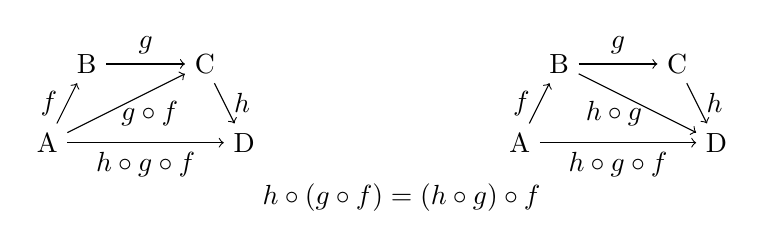
\begin{tikzpicture}
              \node (A) at (-4.5, 0) {A};
              \node (B) at (-4, 1) {B};
              \node (C) at (-2.5, 1) {C};
              \node (D) at (-2, 0) {D};

              \draw[->] (A) edge node[left] {$f$} (B) (B) edge node[above] {$g$} (C)
                        (C) to node[right]{$h$} (D);
              \draw[->] (A) to node[below] {$h \circ g \circ f$} (D);
              \draw[->] (A) to node[pos=0.7, below] {$g \circ f$} (C);

              \node (A) at (1.5, 0) {A};
              \node (B) at (2, 1) {B};
              \node (C) at (3.5, 1) {C};
              \node (D) at (4, 0) {D};

              \draw[->] (A) edge node[left] {$f$} (B) (B) edge node[above] {$g$} (C)
                        (C) to node[right]{$h$} (D);
              \draw[->] (A) to node[below] {$h \circ g \circ f$} (D);
              \draw[->] (B) to node[pos=0.3, below] {$h \circ g$} (D);

              \node at (0, -0.7) {$h \circ (g \circ f) = (h \circ g) \circ f$};
            \end{tikzpicture}
            \end{center}

          \item neutrality :

            \begin{center}
            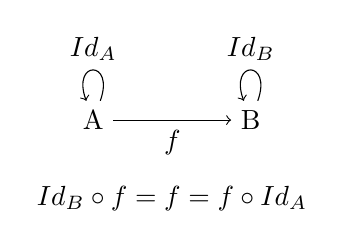
\begin{tikzpicture}
              \node (A) at (-1, 0) {A};
              \node (B) at (1, 0) {B};

              \draw[->] (A) to[out=70,in=110,looseness=8] node[above] {$Id_A$}(A);
              \draw[->] (B) to[out=70,in=110,looseness=8] node[above] {$Id_B$}(B);
              \draw[->] (A) to node[below] {$f$} (B);

              \node at (0, -1) {$Id_B \circ f = f = f \circ Id_A$};
            \end{tikzpicture}
            \end{center}
        \end{itemize}
    \end{itemize}

  \define A small category is a category whose class of object is a set.
  What we defined as a category is called ``\underline{locally small category}''.

  \ex

  \underline{Ordered Set}: Every ordered set $A$ defines a category.
    \begin{itemize}
      \item Objects: elements of $A$
      \item Morphisms : $a \to b \Leftrightarrow a \leq b$
        \[ Hom(a, b) =
          \begin{cases}
            \text{singleton} & a \leq b \\
            \emptyset
          \end{cases} \]

      The composition is defined by transitivity:

        \begin{center}
          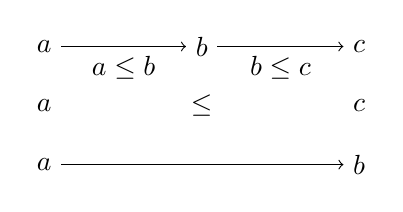
\begin{tikzpicture}
          \node (a) at (-2, 0) {$a$};
          \node (b) at ( 0, 0) {$b$};
          \node (c) at ( 2, 0) {$c$};

          \draw[->] (a) edge node[below] {$a\leq b$} (b)
                    (b) edge node[below] {$b\leq c$} (c);
          ;
          \node at (-2, -0.75) {$a$};
          \node at ( 0, -0.75) {$\leq$};
          \node at ( 2, -0.75) {$c$};
          \node (a) at (-2, -1.5) {$a$};
          \node (b) at ( 2, -1.5) {$b$};
          \draw[->] (a) edge (b);
        \end{tikzpicture}
        \end{center}
    \end{itemize}

    \define An ordered category $\mathcal C$ is a category where $Hom(A,B)$ is a
    singleton for all object $A, B $ of $\mathcal C$.

    \obs An ordered category is the same thing as a pre-order ($=$ trans, refl).

    \ex \underline{Monoid}
    \begin{itemize}
      \item A category with one object $*$, $M = Hom(*, *)$ define a monoid.
        \begin{itemize}
          \item $\circ : Hom(*, *) \times Hom(*,*) \to Hom(*, *)$
          \item $id_* \in M = Hom(*, *)$ define the neutral element
        \end{itemize}
      \item Conversely every monoid $M = (M, \bullet, e)$ defines a category
        $\mathcal B M$ or $\Sigma M$ with:
        \begin{itemize}
          \item One object $*$
          \item $Hom(*, *) = M$
          \item Composition defined by $y \circ x = y \bullet x$ with $e$, the neutral
        element.

        \end{itemize}

      \begin{center}
      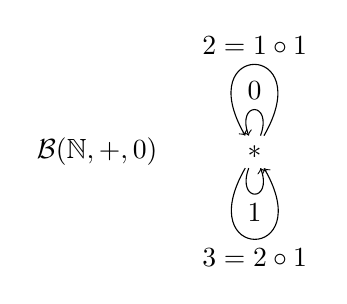
\begin{tikzpicture}
        \node at (-2, 0) {$\mathcal B (\mathbb N, +, 0)$};

        \node (*) at (0, 0) {$*$};

        \draw[->] (*) edge[out=70, in=110, looseness=8]  node[above] {0} (*);
        \draw[->] (*) edge[out=250,in=290, looseness=8]  node[below] {1} (*);
        \draw[->] (*) edge[out=60, in=120, looseness=15] node[above] {$2=1\circ 1$} (*);
        \draw[->] (*) edge[out=240,in=300, looseness=15] node[below] {$3=2\circ 1$} (*);
      \end{tikzpicture}
      \end{center}
    \end{itemize}

  \section{Functors}

    A functor $F : \mathcal A \to \mathcal B$ between category $\mathcal A$ and
    $\mathcal B$ is a graph homomorphism :
    \begin{itemize}
      \item $F$ associates an object $FA$ in $\mathcal B$ to every object $A$
        in $\mathcal A$
      \item $F$ associates a morphism $FA \xrightarrow{Ff} F A'$ in $\mathcal
        B$ to every morphism $A \xrightarrow{f} A'$ in $\mathcal A$.
    \end{itemize}
    It preserves composition and identity

    \begin{center}
    \begin{tikzpicture}
      \node (Aa)  at (-2, -0.7) {$A$};
      \node (Aa') at (-2,  0.7) {$A'$};
      \draw[->] (Aa) to node[right] (f) {$f$} (Aa');
      \draw (-2, 0) ellipse (0.7cm and 1.5cm);

      \node (FAa)  at (2, -0.7) {$FA$};
      \node (FAa') at (2,  0.7) {$FA'$};
      \draw[->] (FAa) to node[left] (Ff) {$Ff$} (FAa');
      \draw (2, 0) ellipse (0.7cm and 1.5cm);

      \draw[|->] (Aa) to (FAa);
      \draw[|->] (Aa') to (FAa');
      \draw[|->] (f) to (Ff);
      
      \node (A)   at (3, -5) {$A$};
      \node (A')  at (3, -4) {$A'$};
      \node (A'') at (3, -3) {$A''$};
      \draw[->] (A)  edge node[left] {$f$} (A')
                (A') edge node[left] {$g$} (A'');

      \node (FA)   at (5.5, -5) {$FA$};
      \node (FA')  at (5.5, -4) {$FA'$};
      \node (FA'') at (5.5, -3) {$FA''$};
      \draw[->] (FA)  edge node[right] {$Ff$} (FA')
                (FA') edge node[right] {$Fg$} (FA'');

      \draw[->] (A)  to (3.5,  -5) to node[right] {$g\circ_A f$} (3.5, -3) to (A'');
      \draw[->] (FA) to (6.2, -5) to node[right]
                {$F g\circ_b F f = F(g \circ_A f)$} (6.2, -3) to (FA'');

      \node (A1)  at (-5, -5) {$A$};
      \node (A2)  at (-5, -3) {$A$};
      \node (FA1) at (-3, -5) {$FA$};
      \node (FA2) at (-3, -3) {$FA$};

      \draw[->] (A1) to node[right] {$Id_A$} (A2);
      \draw[->] (FA1) to node[right] {$F(Id_A) = Id_{FA}$} (FA2);
    \end{tikzpicture}
    \end{center}

  \ex List of different application :
  \begin{itemize}
    \item A Functor $F : \mathcal A \to \mathcal B$ between order category
      is a same thing as a monotone (=order preserving) function. The reason is
      that the preservation of composition and identity holds in $\mathcal B$.
    \item A functor $F : \mathcal B M \to \mathcal B N$ between categories with
      one object is a function $H \to M$ which defined monoid homomorphism.

      $$F(m \circ_M n) = F m \circ_N Fn$$

    \item  functor $F : \mathcal B M \to$ \textit{Set} is a same thing as a
      \textit{Set} $X = F(*)$ equipped with a family of functions $F_m : X \to
      X$ satisfying the equation :
      \begin{itemize}
        \item $F m \circ F n = F (m \bullet n)$
        \item $F(e) = Id_X$
      \end{itemize}
      $\hookrightarrow$ Equivalently a function
      \begin{align*}
        M \times X &\mapsto X \\
        (m, x) &\to m \bullet x
      \end{align*}

      Where we write $F_m(x) = m \bullet x$ and \underline{action} of Mon X
      satisfying the equations of $(m \bullet_M n) \bullet x = m \bullet
      (m \bullet x)$ and $e \bullet x$.

      \ex Given a finite set $A$ (alphabet) of letters. We construct the monoid
      $A^*$ of finite words on $A$  equipped with concatenation as composition
      and empty element as neutral element. We write $[a_1\ldots a_n] \in A^*$
      and $\epsilon$ : the empty word noted $[]$. A functor $\mathcal B A^*
      \xrightarrow{F}$ \textit{Set} is a set $Q = F(*)$ equipped with an action
      that it a function :

      \begin{align*}
        A^* \times Q &\to Q \\
        ([w], q) &\to [w] \bullet q
      \end{align*}

      \remk this action $A \times Q \to Q$ is equivalent to the data of  a
      family $\delta_a : Q \to Q$ of function called transition function of a
      deterministic total automata with \text{Set} of $Q$ of states.

      \exe Given a functor $\mathcal B M \to$ \textit{Set} construct a category
      $\int F$ (Grothendieck construction) whose object are the elements of
      $F(*)$, whose morphisms $x \xrightarrow{m} y$ are of the form $x \mapsto m
      \bullet x$. Show that $\int F$ comes with a functors $\pi : \int F \to
      \mathcal B M$.
    \end{itemize}

  \section{Transformation}
    
    Suppose given functors $F, G : \mathcal A \to \mathcal B$ we want to
    ``compare'' $F$ and $G$ in the same way as we compare two monotone
    functions $f, g: (A, \leq_A) \to (B \leq_g)$ between ordered set.

    \underline{In ordered Set we have} :

      \begin{center}
      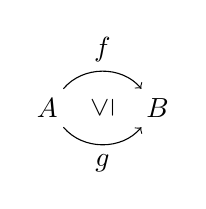
\begin{tikzpicture}
        \node (A) at (-0.7, 0) {$A$};
        \node (B) at ( 0.7, 0) {$B$};

        \node[rotate=90] at ( 0, 0) {$\leq$};

        \draw[->] (A) to[bend right=50] node[below] {$g$} (B);
        \draw[->] (A) to[bend left =50] node[above] {$f$} (B);
        \end{tikzpicture}
      \end{center}
      $$f \leq_A g \Leftrightarrow \forall a \in A, f(a) \leq_B g(a)$$

      \define A transformation $\theta : F \Rightarrow G : \mathcal A \to
      \mathcal B$ is a family of morphisms $\theta : FA \to GA$ in $\mathcal B$
      parametrised by the object $A$ of $\mathcal A$

      \nota We write :
      \begin{center}
      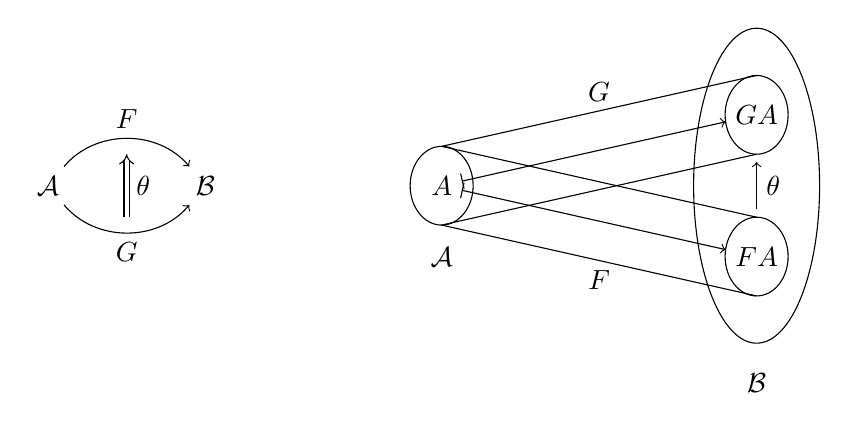
\begin{tikzpicture}
        \node (A) at (-1, 0) {$\mathcal A$};
        \node (B) at ( 1, 0) {$\mathcal B$};

        \draw[->] (A) to[bend right=50] node[below] {$G$} (B);
        \draw[->] (A) to[bend left =50] node[above] {$F$} (B);
        \draw[double equal sign distance, -implies] (0, -0.4) to node[right]
          {$\theta$} (0, 0.4);

        \draw (4, 0) ellipse (0.4cm and 0.5cm);
        \node (A) at (4, 0) {$A$};
        \node at (4, -0.9cm) {$\mathcal A$};

        \draw (8,  0.9) ellipse (0.4cm and 0.5cm);
        \draw (8, -0.9) ellipse (0.4cm and 0.5cm);
        \node (GA) at (8,  0.9) {$GA$};
        \node (FA) at (8, -0.9) {$FA$};

        \draw (8, 0) ellipse (0.8cm and 2cm);
        \node at (8, -2.5cm) {$\mathcal B$};

        \draw (4,  0.5cm) -- node[above] {$G$} (8, 1.4cm);
        \draw (4, -0.5cm) -- (8, 0.4cm);

        \draw (4,  0.5cm) -- (8, -0.4cm);
        \draw (4, -0.5cm) -- node[below] {$F$} (8, -1.4cm);

        \draw[->] (8, -0.3) to node[right] {$\theta$} (8, 0.3);

        \draw[|->] (A) to (GA);
        \draw[|->] (A) to (FA);
      \end{tikzpicture}
      \end{center}

      \fact Every pair of categories $\mathcal A, \mathcal B$ defined a
      category \textit{Trans}$(\mathcal A, \mathcal B)$ object are functors $F: A
      \to B$ and morphism are transformation $\theta : F \Rightarrow G$.

      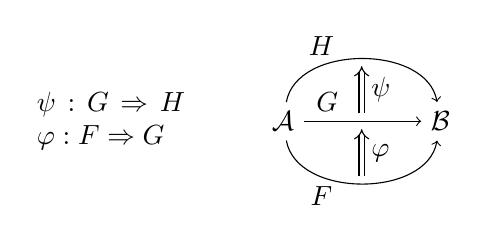
\begin{tikzpicture}
        \node[text width=2.25cm] at (0, 0) {$\psi : G \Rightarrow H$
        $\varphi : F \Rightarrow G$};

        \node (A) at (2, 0) {$\mathcal A$};
        \node (B) at (4, 0) {$\mathcal B$};

        \draw[->] (A) edge[bend right=80] node[below, pos=0.3] {$F$} (B);
        \draw[->] (A) edge node[above, pos=0.2] {$G$} (B);
        \draw[->] (A) edge[bend left =80] node[above, pos=0.3] {$H$} (B);
        \draw[double equal sign distance, -implies]
          (3, 0.1) to node[right] {$\psi$} (3, 0.7);

        \draw[double equal sign distance, -implies]
          (3, -0.7) to node[right] {$\varphi$} (3, -0.1);
      \end{tikzpicture}

      The composite transposition it's easy to define $(\psi \circ \varphi)_A =
      \psi_A \circ \varphi_A$ and the identity is $Id_F : F \Rightarrow F$
      $(Id_F)_A = Id_{FA}$.

      We can write this :

      \begin{center}
      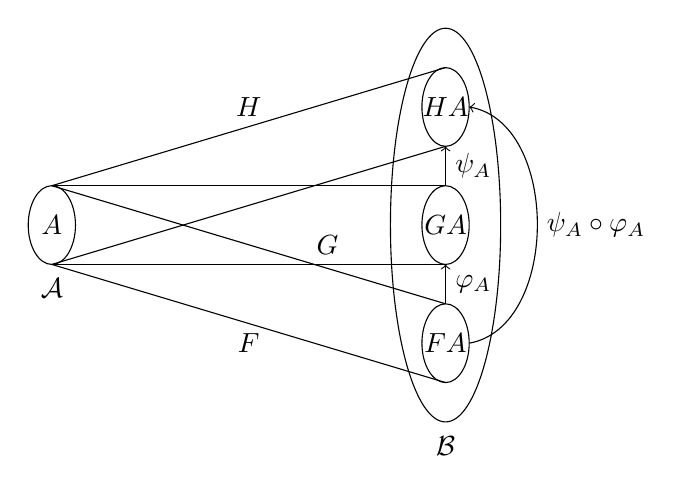
\begin{tikzpicture}
        \coordinate (A) at (0, 0);
        \coordinate (B) at (5, 0);

        \draw (A) ellipse (0.3cm and 0.5cm);
        \node at (A) {$A$};
        \node at (0, -0.8) {$\mathcal A$};

        \draw (B) ellipse (0.7cm and 2.5cm);
        \node at (5, -2.8) {$\mathcal B$};

        \draw (5, 1.5) ellipse (0.3cm and 0.5cm);
        \node (HA) at (5, 1.5) {$HA$};
        \draw (5, 0) ellipse (0.3cm and 0.5cm);
        \node (GA) at (5, 0) {$GA$};
        \draw (5, -1.5) ellipse (0.3cm and 0.5cm);
        \node (FA) at (5, -1.5) {$FA$};

        \draw (0, 0.5cm) -- node[above] {$H$} (5, 2);
        \draw (0, -0.5cm) -- (5, 1);

        \draw (0, 0.5cm) -- (5, 0.5);
        \draw (0, -0.5cm) -- node[above, pos=0.7] {$G$} (5, -0.5);

        \draw (0, 0.5cm) -- (5, -1);
        \draw (0, -0.5cm) -- node[below] {$F$} (5, -2);

        \draw[->] (5, -1) to node[right] {$\varphi_A$} (5, -0.5);
        \draw[->] (5, 0.5) to node[right] {$\psi_A$} (5, 1);
        \draw[->] (5.3, -1.5) to[bend right=80] node[right]
                  {$\psi_A \circ \varphi_A$} (5.3, 1.5);
      \end{tikzpicture}
      \end{center}

  \subsection{Post-composition}
  
    \supo Given a transformation $\varphi : F \Rightarrow G : \mathcal A \to
      \mathcal B$ and a functor $H : \mathcal B \to \mathcal C$

      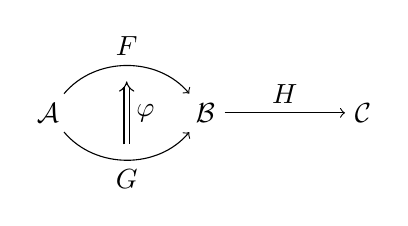
\begin{tikzpicture}
        \node (A) at (2, 0) {$\mathcal A$};
        \node (B) at (4, 0) {$\mathcal B$};
        \node (C) at (6, 0) {$\mathcal C$};

        \draw[->] (A) edge[bend right=50] node[below] {$G$} (B);
        \draw[->] (A) edge[bend left =50] node[above] {$F$} (B);
        \draw[double equal sign distance, -implies]
          (3, -0.4) to node[right] {$\varphi$} (3, 0.4);
        \draw[->] (B) edge node[above] {$H$} (C);
      \end{tikzpicture}

      We define the transformation

      \begin{align*}
        H \circ_l \varphi_A &: \mathcal A \mapsto \varphi \\
        & H F A \to H G A
      \end{align*}

      We can represent this transformation like this :

      \begin{center}
      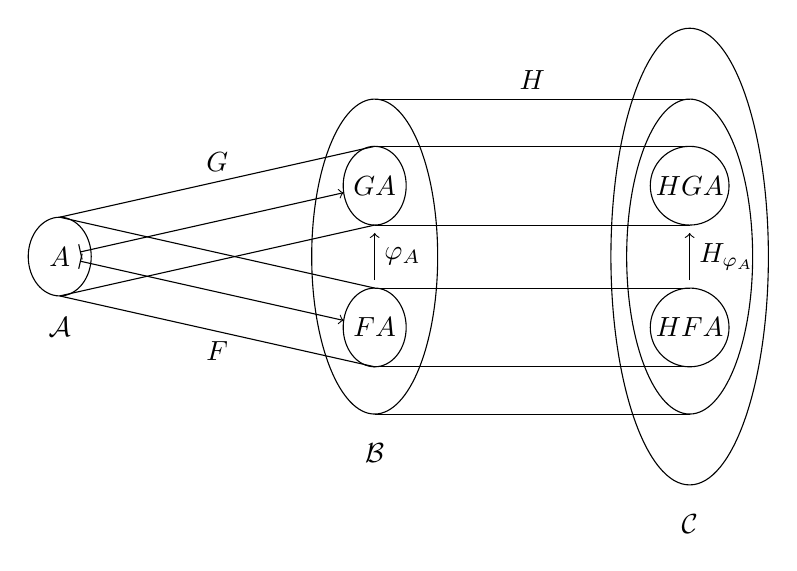
\begin{tikzpicture}
        \draw (4, 0) ellipse (0.4cm and 0.5cm);
        \node (A) at (4, 0) {$A$};
        \node at (4, -0.9cm) {$\mathcal A$};

        \draw (8,  0.9) ellipse (0.4cm and 0.5cm);
        \draw (8, -0.9) ellipse (0.4cm and 0.5cm);
        \node (GA) at (8,  0.9) {$GA$};
        \node (FA) at (8, -0.9) {$FA$};

        \draw (8, 0) ellipse (0.8cm and 2cm);
        \node at (8, -2.5cm) {$\mathcal B$};

        \draw (4,  0.5cm) -- node[above] {$G$} (8, 1.4cm);
        \draw (4, -0.5cm) -- (8, 0.4cm);

        \draw (4,  0.5cm) -- (8, -0.4cm);
        \draw (4, -0.5cm) -- node[below] {$F$} (8, -1.4cm);

        \draw[->] (8, -0.3) to node[right] {$\varphi_A$} (8, 0.3);

        \draw[|->] (A) to (GA);
        \draw[|->] (A) to (FA);

        \draw (12,  0.9) ellipse (0.5cm and 0.5cm);
        \draw (12, -0.9) ellipse (0.5cm and 0.5cm);
        \node (HGA) at (12,  0.9) {$HGA$};
        \node (HFA) at (12, -0.9) {$HFA$};

        \draw (12, 0) ellipse (0.8cm and 2cm);
        \draw (12, 0) ellipse (1cm and 2.9cm);
        \node at (12, -3.4cm) {$\mathcal C$};

        \draw (8, 1.4cm) -- (12, 1.4cm);
        \draw (8, 0.4cm) -- (12, 0.4cm);

        \draw (8, -0.4cm) -- (12, -0.4cm);
        \draw (8, -1.4cm) -- (12, -1.4cm);

        \draw (8, 2cm) -- node[above] {$H$} (12, 2cm);
        \draw (8, -2cm) -- (12, -2cm);

        \draw[->] (12, -0.3) to node[right] {$H_{\varphi_A}$} (12, 0.3);
      \end{tikzpicture}
      \end{center}

    \subsection{Pre-composition}

\end{document}
